\cotefile{15}
\scanpage{34}
% archive foliation: 33

\uline{Ex. 3} Soit fixé, en plus de la catégorie de Deuring $C$ sur $A$ comme dans Ex. 2, un élément $\tau$ de $V_A(C)$. Si $E$ est \inserted{\unsure{centrale}} de rang $n$, il faut considérer que les $C$ qui \uline{\unsure{réalisent}} les
\deleted{(\unsure{de manière à convenir à la rigueur})}
\unsure{gerbes} de lien $G_m$ \uuline{sur $A$} trivialisées par $n$,
\deleted{et \unsure{sur} $A$ (car si $E$ est \unsure{définie} sur $A$ \unsure{complète de} \unsure{$G_m$})}
\inserted{$C$ qui correspond au \unsure{corps} \deleted{\unsure{grp}}, \unsure{dans $K$}, cela revient à une algèbre d'Azumaya sur $R$, i.e. la classe de $E$ dans $\mathrm{Br}(K)$ est dans l'image de $\mathrm{Br}(R)$.}
et il faut voir de \unsure{même} que les couples $(C,\tau)$ \unsure{équivalent} à la donnée d'une gerbe de groupe $\mu_n$.

\margin{\unsure{et trivialisation}\\
\unsure{gerbes} sur $A$ de lien $G_m$ $\longrightarrow$ catégorie $C$ des \unsure{représentations} \unsure{faisant} \unsure{des} \unsure{objets} \unsure{fidèles} \unsure{vis-à-vis} du groupe, poids $1$.}
\margin{$C\longmapsto$ \unsure{gerbes} des foncteurs admissibles de $C$ dans les \unsure{modules} \unsure{``caractéristiques''} de $C$\\
cat. de Deuring sur \unsure{$E$}\\
\unsure{$\longleftarrow$} \unsure{$\xi\in\widehat{\mathcal G}$}\\
\unsure{$\widehat{\mathcal G}=[\mathrm{Br}\,A\longrightarrow\mathrm{Br}\,K]$}}

Pour cela, \deleted{\unsure{on}} introduire \deleted{\unsure{la catégorie des gerbes}} pour une gerbe de lien $\mu_n$ sur $A$ \unsure{définir} bien une $(C,\tau)$:

$C$: les \deleted{\unsure{trivialisations}} \deleted{de} \unsure{représentations} de degré $n$, de rang $1$ dans la gerbe, $\tau=$ \deleted{\unsure{la représentation déterminant}}.

Nous allons déterminer d'abord \unsure{quels sont} les autoéquivalences de $(E,\tau)$; en termes d'un objet $X$ de $C$, \inserted{d'où $O=\operatorname{End}(X)$,} c'est la catégorie des \deleted{\unsure{algèbres}} bimodules $P$ \unsure{sous} $O$, inv. loc. sur $A$ des deux côtés, munis d'un isom
\[
N_{O/A}(P_{\unsure{O|\sigma}})\simeq\deleted{\unsure{O}}A.
\]
\inserted{dans $P(A)$}
\margin{(\deleted{$\unsure{\nu}(X)=L\otimes$} $\tau=L\otimes_A\nu(X)$)}
\margin{\[
\begin{aligned}
\varphi(X)&=P\otimes_O X\\
\nu(\varphi(X))&=N(P)\otimes\nu(X)\\
&\unsure{\simeq}\\[-6pt]
&\varphi(\nu(X))
\end{aligned}
\]}
\deleted{\unsure{compatible avec}}

\deleted{Supposons que tous les $P_{\unsure{O|\sigma}}$ \inserted{\unsure{de} $\unsure{P(O/A)}$} soient isomorphes, ce qui est le cas si $A$ est local, \unsure{ou} semi local.}

\unsure{Alors} c'est une Gr.-catégorie, \inserted{et \unsure{même} une catégorie de Picard \unsure{str. comm.}} \unsure{où} les endom. de l'objet $1$ sont les éléments $\lambda\in A^*$ tels que $\lambda^n=1$; \unsure{cette} catégorie de Picard contient comme sous-catégorie pleine $\uline{\operatorname{Tors}}(S,\mu_n)$ des

\scanpage{36}
% archive foliation: 35

torseurs sur $S$ de groupe $\mu_n$, et son $\pi_1$ \deleted{\unsure{est}} s'insère dans
\diagram{\begin{tikzcd}
0 \arrow[r] & \unsure{H^1(S,\mu_n)} \arrow[r] &
\pi_0(\uline{\operatorname{Brdt}}(C,\tau)) \arrow[r] &
\deleted{\unsure{\mathrm{Br}(C)}}\inserted{\operatorname{Ram}(C/A)} \arrow[r] & 0 .
\end{tikzcd}}
\deleted{(Si $\operatorname{Pic}(A)=0$, \unsure{cette catégorie}}
\[
\text{\uline{où}}\quad
\operatorname{Ram}(C/A)
\underset{\deleted{\unsure{=}}}{\overset{\mathrm{déf}}{=}}
\unsure{\operatorname{Brdt}}(C)/\operatorname{Pic}(A)
\simeq\sum_{\mathfrak p}\mathbb Z/e_{\mathfrak p}(C)\mathbb Z.
\]
\margin{$e_{\mathfrak p}(C)$: degré de ramification}

\deleted{Mais} Soit maintenant $A'$ une $A$-algèbre (comm.)
\deleted{Dans le cas}
et $C'$ une catégorie de Deuring sur $A'$, \inserted{et $T'\in V_{\unsure{A'|A}}(C')$,}
\unsure{supposons} $(C_{A'},T_{A'})\underset{A'}{\simeq}(C',\unsure{T'|A'})$.
\deleted{Alors l'ensemble des}
(il suffit pour ceci que $C_{A'}\simeq C'$ et $\operatorname{Pic}(A')=0$, p. ex. $A'$ local)
Alors l'ens. des équivalences de $(C_{A'},T_{A'})$ vers $(C',T')$, i.e. des couples $(\varphi,u)$ avec $\varphi$
\deleted{\unsure{équivalence}}
\diagram{\begin{tikzcd}
C_{\unsure{A'}} \arrow[r,"\varphi"] & C'
\end{tikzcd}}
\deleted{\unsure{de}} $A$-linéaire \unsure{admis.}, induisant $\simeq C_{A'}\longrightarrow C'$, et
\[
u:\nu(\varphi)(T_{A'})\xrightarrow{\sim}T',
\]
est une \uline{catégorie} \uline{torseur} sous la \inserted{Gr.-}catégorie
\[
\unsure{\mathrm{Eq}}\ \uline{\mathrm{Eq}}(C_{A'},T_{A'})
\quad\text{(à droite)}\quad
\text{\unsure{et}}\quad
\uline{\mathrm{Eq}}(C',T')\quad\text{(à gauche)}.
\]

Si p. ex. $\operatorname{Ram}(C'/A')=0$ ($C'$ non ramifiée sur $A'$)
\deleted{\unsure{on doit}} alors c'est une catégorie-torseur sous
\deleted{\unsure{$\mathcal E$}} $\uuline{\operatorname{Tors}}(S',\mu_n)$.
En fait, \unsure{on a} une équivalence \uline{canonique}
\[
\uline{\mathrm{Eq}}(C_{A'},T_{A'})
\simeq
\uline{\mathrm{Eq}}(C',T')
\]
(comme une \deleted{\unsure{Gr.-}} catégorie de \uuline{Picard}) et par suite les deux structures de tors.-catégories \unsure{peuvent} s'identifier \unsure{\ldots}
\margin{\uuline{À vérifier!!}}

\scanpage{38}
% archive foliation: 37

Supposons qu'on ait pu associer \uline{canoniquement}, à la catégorie de Deuring-Brauer $C$ (en termes de la seule classe d'équivalence de $C$), un objet $T$ de \unsure{$V(C)$}. Cela signifie en particulier que nous avons relevé le foncteur canonique \inserted{de Gr.-cat.}
\diagram{\begin{tikzcd}
\uline{\mathrm{Eq}}(C,T) \arrow[r] &
\uline{\mathrm{Eq}}(C) \arrow[l,bend left=30,swap,"\deleted{\unsure{a}}c"]
\end{tikzcd}}
en

Donc pour tte catégorie $C'$ équivalente à $C$, on obtient un objet $T_{\unsure{C'}}^{\unsure{c}}$ canonique dans $V(C')$.
On voit donc que pour tt $(A',C',T')$ comme plus haut, \deleted{l'ensemble} tel que $(C',T')$ est équivalent à $(C,T)_{A'}$, les équivalences en question font une \uline{catégorie-torseur} sous
\[
\uline{\mathrm{Eq}}((C,T)_{A'})
\inserted{\simeq\uline{\mathrm{Eq}}(C',T')},
\]
\deleted{donc définissent une catégorie torseur sous
$\uline{\mathrm{Eq}}(C',T')/\inserted{\operatorname{Im}}\uline{\mathrm{Eq}}(C)$ par passage}
les classes d'isom d'objets font un torseur sous
$\unsure{\operatorname{Brd}|\operatorname{Brdt}}(C',T')$,
donc définissent un torseur sous
\[
\unsure{\operatorname{Brd}|\operatorname{Brdt}}(C',T')/
\operatorname{Im}\unsure{\operatorname{Brd}|\operatorname{Brdt}}(C).
\]
Le torseur ne dépend plus du choix d'un $C$ dans la classe de catégories envisagées\ldots
Il faut donc expliciter l'application composée
\diagram{\begin{tikzcd}[column sep=large]
\unsure{\operatorname{Brd}}(C) \arrow[r,"c"] &
\unsure{\operatorname{Brd}}(C,T) \arrow[r] &
\unsure{\operatorname{Brd}}(C',T')\\
\rho \arrow[r,mapsto] &
(\rho,u_\rho) \arrow[r,mapsto] &
(\rho',u_{\rho'})\\
\unsure{P_O} \arrow[r,mapsto] \arrow[u,phantom,"\unsure{\simeq}"] &
N_{O/A}(\unsure{P_O})\unsure{\ni}u_\rho \arrow[r,mapsto] &
N_{O'/A'}(\unsure{P'_{O'}|P'_O})\unsure{\ni}(u_\rho)'
\end{tikzcd}}

\scanpage{40}
% archive foliation: 39

Dans le cas qui nous intéresse ($\unsure{\zeta}\in\mathrm{Br}(\mathbb Q)$ d'indice $n=2$, ramifié exactement en $\unsure{2|p}$ et $\infty$) \deleted{\unsure{on trouve}}
on trouve que $\unsure{\operatorname{Brd}}(C)$ est la \deleted{groupe} \inserted{catégorie} de Picard splittée d'invariants $\mathbb Z/2\mathbb Z$, $\mathbb Z/2\mathbb Z$, le générateur $\rho$ de $\pi_0$ \unsure{correspond} au \deleted{\unsure{l'endomorphisme}} foncteur qui à une courbe elliptique $E$ associe $E^{(p)}=E/\operatorname{Ker}F_E$)
correspond à l'unique idéal premier $\mathfrak m$ de $O$ sur $p$, et on a
\diagram{\begin{tikzcd}
N_{O/\mathbb Z}(\mathfrak m) \arrow[r] \arrow[d,phantom,"\parallel"] &
N_{O/\mathbb Z}(O)=\mathbb Z\\
p\mathbb Z &
\end{tikzcd}}
, on choisit $\bar\rho=p$.

Ceci nous dit que \uline{si $p$ est inversible dans} $A'$, alors l'image de $(\rho,\bar\rho)$ dans
\[
\unsure{\operatorname{Brd}}(C_{A'},T_{A'})
\simeq\deleted{\unsure{\operatorname{Brd}(C_{A'})}}
H^1(S',\mu_2)
\]
est la \unsure{classe} de $p$ modulo des carrés.

Par contre, prenons le cas où $A'=\mathbb Z_p$, alors
\deleted{\unsure{on est dans un groupe}}
\[
\unsure{\operatorname{Brd}}(C'_p,T'_p)
\simeq\unsure{\operatorname{Brd}}(C_{A'},T_{A'})
\]
est une extension de $\mathbb Z/2\mathbb Z$ par
$\mathbb Z_p^*/\mathbb Z_p^{*2}$
($\simeq\mathbb Z/2\mathbb Z$ si $p\ne2$), en fait c'est
\[
\underbrace{\mathbb Z_p^*/\mathbb Z_p^{*2}}_
{\parallel\ H^1(\mathbb Z_p,\mu_2)\ \deleted{\unsure{(\mathbb Z_p,A)}}}
\times
\underbrace{\mathbb Z/2\mathbb Z}_{\text{engendré par }(\mathfrak m,p)},
\]
\margin{$C_p=C'$\\$T_p=T'$}
et les classes d'isom possibles des \inserted{(du moins à l'$\infty$)}
\deleted{\unsure{liens}}
forment un torseur sur ce groupe
(\deleted{\unsure{le plus grand}}
$\simeq\mathbb Z/2\mathbb Z\times\mathbb Z/2\mathbb Z$ si $p\ne2$).

D'autre part, si $A'=\mathbb R$, on peut considérer les classes d'isomorphie de la gerbe de lien $\mu_2$ sur $\mathbb R$ définie par $C$ (soit $\unsure{\mathfrak g}_{\mathbb R}$, où $\unsure{\mathfrak g}$ est la gerbe sur $\mathbb Z[1/p]$) et l'ensemble des classes d'\inserted{\unsure{morphismes d'}}équivalences avec la gerbe \unsure{type} sur $\mathbb R$ ($=$ ensemble des \uline{\unsure{plexions|flexions}} de la gerbe), qui est un torseur sous
\[
H^1(\mathbb R,\mu_2)=\mathbb R^*/\mathbb R^{*2}.
\]
On trouve donc

\scanpage{42}
% archive foliation: 41

Si on se donne la \deleted{gerbe} \inserted{catégorie de Deuring \unsure{rigidifiée|associée}}
$(C'(A'),T')$ sur $A'=\prod_{\ell\ne p,\infty}\mathbb Z_\ell$ comme associée à la gerbe des racines carrées de $A'(1)$ (définie par le choix d'une clôture algébrique $\overline{\mathbb F}_p$ de $\mathbb F_p$), et la catégorie de Deuring $C(\mathbb Z_p)$ comme celle des $F$-cristaux sur $\overline{\mathbb F}_p$ (à iso) qui sont de rang $2$, \deleted{\unsure{tous}} pente $\frac12$, \inserted{avec le foncteur de Tate}, et la \deleted{gerbe}
catégorie $C(\mathbb Z_\infty)=C(\mathbb R)$ comme associée à la gerbe type $\unsure{\mathfrak g}_\infty$ de groupe $\mu_2$ sur $\mathbb R$, on trouve un \unsure{torseur}
\deleted{\unsure{\mathcal T}(C)} un certain torseur \inserted{$\mathcal T'(C)$} sous le groupe
\[
\deleted{\unsure{\mathbb Z_p}}\quad
A'^*/A'^{*2}\times
(\mathbb Z_p^*/\mathbb Z_p^{*2}\times\mathbb Z/2\mathbb Z)
\times\mathbb R^*/\mathbb R^{*2}=\Gamma'.
\]

Le groupe \inserted{$\mathbb Z/2\mathbb Z$} des classes d'isomorphie d'autoéquivalences de \deleted{$C$} opère sur ce torseur, de façon compatible avec son opération triviale sur lui-même, donc par translations, et il opère donc via un hom. \inserted{$f$ (\unsure{l'hyp. scindée})} de $\mathbb Z/2\mathbb Z$ dans ce groupe,
\deleted{\unsure{dont les}} l'image du \inserted{gén.} $f$ de $\mathbb Z/2\mathbb Z$ dans les $3$ facteurs étant respectivement
\[
(p,\ \unsure{\beta}=(0,1),\ p)
\]
\margin{N.B. \inserted{Comme $p\in\mathbb R^{*2}$}
\deleted{\unsure{on peut donc}, \unsure{elle est négligeable}, \unsure{dans}}
l'ens. des \unsure{plexions},
\deleted{\unsure{distinguer canoniquement le}}
$\unsure{\mathrm{Pl}}(C)$ il y a un système transitif d'isomorphismes!}

Considérons le quotient
\[
\Gamma=\Gamma'/f(\pm1),
\]
\deleted{On \unsure{voit donc}}
et soit $\mathcal T(C)$ le quotient de $\mathcal T'(C)$ par $\pm1$, qui est donc un torseur sous $\Gamma$.
Ce torseur, à isom unique près, ne dépend pas de $C$, \inserted{on peut l'appeler $\mathcal T$ ou $\mathcal T(\overline{\mathbb F}_p)$,}
D'ailleurs si $\Gamma'_0$ est le ss-grp de $\Gamma'$
\[
A'^*/A'^{*2}\times\mathbb Z_p^*/\mathbb Z_p^{*2}
\times\mathbb R^*/\mathbb R^{*2}
=H^1_{\deleted{\unsure{\mathrm{ét}}}}(\mathbb A,\mu_2)
\]
\margin{adèles}
on trouve que $\Gamma'\simeq\Gamma'_0\times f(\pm1)$, donc $\Gamma\simeq\Gamma'_0$ (can., donc

\scanpage{44}
% archive foliation: 43

$\mathcal T(\overline{\mathbb F}_p)$ est un torseur canonique sous
\[
\begin{gathered}
H^1(\mathbb A,\mu_2)\\
\parallel\\
\prod_{\ell}\mathbb Z_\ell^*/\mathbb Z_\ell^{*2}\\
\text{(y compris $p$ et $\infty$)}
\end{gathered}
\]

Ce torseur à priori dépend encore de $\overline{\mathbb F}_p$, \deleted{\unsure{on doit donc}} et cette dépendance est précisée par la connaissance de l'opération de $\widehat{\mathbb Z}\ni f$ sur $\mathcal T(\overline{\mathbb F}_p)$.
Cette opération se fait via les opérations de $\widehat{\mathbb Z}$ sur $C(A',T')$,
\inserted{(opère \unsure{habituellement} sur $A'(1)$, $f$ opère par $p$) et}
\deleted{\unsure{$C(A_p,T_p)$}}
\inserted{$C(A_p,T_p)$}
(via opération de $\deleted{\unsure{\mathbb Z}}\mathbb Zf$ sur $C(A_p,T_p)$ par Frobenius) et l'opération triviale sur $C(A_\infty,T_\infty)$.
Donc on trouve que $f\in\widehat{\mathbb Z}$ opère par le même élément $(p,f,p)$ que plus haut, donc
\[
f\text{ opère trivialement sur }\mathcal T(\overline{\mathbb F}_p)
\]
Ainsi, on a un torseur canonique \inserted{$\mathcal T$} sous $H^1(\mathbb A,\mu_2)$.

\uline{NB} Ceci suggère qu'on a une \deleted{\unsure{gerbe de catégories}} \inserted{gerbe triviale (ou} \unsure{trivialisée)} de \deleted{\unsure{faisceaux}} $\mu_2$ sur $\mathbb A$, dont $\mathcal T$ serait le torseur des classes d'isomorphie.
On peut en effet considérer les couples $(C,\deleted{\unsure{\xi}}\alpha)$, où $C$ est une catégorie de Deuring de type $\xi\in\mathrm{Br}(\mathbb Q)$, \inserted{d'où $T_C=T$,} et $\alpha$ une \deleted{\unsure{isom}} classe d'équivalences de classes d'isomorphie \inserted{\unsure{le privilège}} de $(C,T)_{\mathbb Z_p}$ avec $C(\mathbb Z_p),T(\mathbb Z_p)$ modulo équivalences provenant de $\uline{\operatorname{Pic}}(\mathbb Z_p)$; i.e. une section du torseur de groupe $\mathbb Z/2\mathbb Z$ déduit de celui de groupe
\[
\unsure{\mathrm{Eq}}(C(\mathbb Z_p),T(\mathbb Z_p))
=\mathbb Z_p^*/\mathbb Z_p^{*2}\times\mathbb Z/2\mathbb Z
\]
\unsure{relatif} par \unsure{extension} au groupe \unsure{standard} à l'aide de $\operatorname{pr}_2$.

\margin{\deleted{\unsure{à isom près}}
On \unsure{précise}: (objets: \unsure{quotients} $(M,\sigma)$): \uline{isom} \uline{près}
(il y a deux classes d'isomorphie possibles; si $(M,\sigma)$ est l'une d'elles, l'autre est $(M^{(p)},\sigma)$ \unsure{qui} \unsure{s'en déduit en appliquant} Frobenius).}

\margin{\unsure{plus compliqué}, il suffit de \unsure{fixer une} classe d'isom. près d'équivalences de cat.
$C_{\mathbb Z_p}\simeq C(\mathbb Z_p)$ \unsure{de Deuring}.}
\margin{en termes concrets.
un $\alpha$ est donné ($C$ défini par $O$) en se donnant une \unsure{isom} de $O\otimes_{\mathbb Z}\mathbb Z_p$ avec l'anneau des endom. de $\unsure{M_0}$; où \unsure{$M_0$ est un} cristal sur $\overline{\mathbb F}_p$ (\unsure{de rang $2$}),
\deleted{\unsure{on dispose}\ \unsure{$\widehat A/\widehat A^{\,2}$}\ \illegible{3}}.}

Alors tout $C$ admet un $\alpha$, et deux $(C,\alpha)$ $(C',\alpha')$

\scanpage{46}
% archive foliation: 45

\deleted{sont \uline{\unsure{canoniquement}} équivalentes, \unsure{Si on les} \unsure{couples} essentiellement identifiés entre eux les différents $(C,\alpha)$, on trouve ainsi une catégorie de Deuring \uline{canonique}}
\inserted{l'équivalence canonique à isom près}
sont équivalents: la catégorie des équivalences de $(C,\alpha)$ vers $(C',\alpha')$ est un groupoïde connexe de $\pi_1\quad\mathbb Z/2\mathbb Z$:
i.e. tt d'abord les équivalences sont isom., et si on a deux équiv. $\varphi,\varphi'$, il y a \uline{au signe près} un seul isom. entre $\varphi$ et $\varphi'$.

Si on se donne maintenant un couple $(C,\alpha)$, il lui est associé une \deleted{torseur sur} gerbe sur
$\mathbb A=\prod_\ell\mathbb Z_\ell$ \inserted{(y compris $\ell=p$, $\ell=\infty$)}
\inserted{de groupe $\mu_2$,}
savoir celle des équivalences \inserted{de $(C,T)$} avec le \deleted{gerbe} couple type de $(C(\mathbb A),T)$, qui en la place $p$ soit compatible avec la donnée de $\alpha$.
Cette gerbe, $\unsure{\mathfrak g}_{(C,\alpha)}$ est déterminée, ``à un signe près'' \unsure{à} équivalence unique près, indépendamment du choix de $(C,\alpha)$ (puisqu'il en est ainsi de $(C,\alpha)$ lui-même), \deleted{et}
\deleted{$\unsure{\mathcal T}=\unsure{\mathcal T}(\overline{\mathbb F}_p/\mathbb F_p)$ \unsure{opère trivialement}.}
mais elle dépend à priori \inserted{\unsure{$\simeq$ pour $(C,\alpha)$ fixé},} du choix d'un $\overline{\mathbb F}_p$
\deleted{(ou du moins de $\mathbb F_{p^2}$)}
--- tout comme la structure $\alpha$ elle-même!

\margin{\deleted{\unsure{Cristal} \unsure{isocline} de rang $2$, pente $\frac12$ sur $\overline{\mathbb F}_p$, en descendant \uline{canoniquement} à $\mathbb F_{p^2}$.}}

On peut s'en tirer en définissant \uline{canoniquement} un $\mathbb F_{p^2}$ (ou même un $\overline{\mathbb F}_p$, si on y tenait \ldots) par les polynômes cyclotomiques $\Phi_{p^n-1}$,
\[
\overline{\mathbb F}_p=
\underset{n}{\underrightarrow{\lim}}\,
\bigl(\mathbb F_{p^n}=\mathbb F_p[T]/\Phi_{p^n-1}(T)\bigr)
\qquad\ldots
\]

\scanpage{48}
% archive foliation: 47

Considérons cette gerbe $\unsure{\mathfrak G}$ sur $\mathbb A=\prod_p\mathbb Z_p$, de groupe $\mu_2$, définie ``au signe près'' (de façon précise, on a une $2$-catégorie des $(C,\alpha)$, qui \unsure{satisfait} $\pi_0=\pi_1=0$, $\pi_2=\mathbb Z/2\mathbb Z$, et \deleted{que} on a \deleted{\unsure{une}} \inserted{une famille de gerbes} indexée par $\mathcal D$, i.e. un $2$-foncteur de $\mathcal D$ dans la $2$-catégorie des \deleted{\unsure{$2$-}}gerbes sur $\mathbb A$, groupe $\mu_2$).
Dans cette gerbe, on a une ``\uline{section définie à isom can. au signe près}''.

\margin{attention: \unsure{réalité}, \unsure{s'il n'y a pas} \unsure{un dernier} signe!}

\medskip
\hrule
\medskip

Autre façon d'exprimer: le \deleted{catégorie des \unsure{\operatorname{Eq}}} \inserted{foncteur des} catégories de Picard \unsure{composé}
\diagram{\begin{tikzcd}[column sep=large]
\uline{\mathrm{Eq}}(\unsure{C}) \arrow[r] &
\uline{\mathrm{Eq}}(C,T) \arrow[r] &
\uline{\mathrm{Eq}}(C_p,T_p) \arrow[d,phantom,"\simeq\text{ can.}"]\\
&&\mathrm{Eq}(C(\mathbb Z_p),T(\mathbb Z_p))
\end{tikzcd}}
est pleinement fidèle, la catégorie de Picard quotient est donc une catégorie rigide, qui n'est autre que
$[0\longrightarrow\mathbb Z_p^*/\mathbb Z_p^{*2}]$.
Donc la catégorie des équivalences de $(C,T)_{\mathbb Z_p}$ avec $(C(\mathbb Z_p),T(\mathbb Z_p))$
\uline{modulo action de} $\uline{\mathrm{Eq}}(C)$ est une catégorie rigide,
\deleted{torseur} dont l'ens des classes d'isom. est un $\mathcal T_p$, torseur canonique sous $\mathbb Z_p^*/\mathbb Z_p^{*2}$ (un élément \deleted{lequel}\inserted{privilégié}!!!), indépendant à isom can. près de $C$.
\deleted{On \unsure{a un} \unsure{point} \unsure{can.} $\xi\in\mathcal T_p$.}
\deleted{Après \unsure{avoir choisi} \unsure{le dernier} \unsure{isomorphisme}}
On peut considérer les couples $(C,\alpha)$, où $\alpha$ est une équivalence
\[
(C,T)_{\mathbb Z_p}\simeq(C(\mathbb Z_p),T(\mathbb Z_p))
\]
\uline{dans la classe de} $\xi_p$, et
\deleted{\unsure{on}}
si on a deux tels couples, ils sont \uline{\unsure{isomorphes}} d'une \uuline{façon canonique}.

\scanpage{50}
% archive foliation: 49

Donc on peut \deleted{considérer que} \inserted{identifier} les $(C,\alpha)$ \deleted{sont} entre eux \deleted{\unsure{et tout}}, et trouver un
\[
[C(\xi),\alpha(\xi)]\quad\text{canonique}.
\]

\deleted{On peut alors considérer sur $A''$ \inserted{$=A'\times A_\infty$} (anneau des adèles premières à $p$), la gerbe $g''$ \inserted{de groupe $\mu_2$} qui sur $A'$ est la gerbe des racines carrées de $A'(1)$, et sur $A_\infty$ est la gerbe type $g'_\infty$ déjà envisagée \unsure{plus haut}.}

En fonction de ce choix, on trouve une gerbe canonique $\mathfrak G(\xi)$ sur l'anneau des adèles, de groupe $\mu_2$, savoir la gerbe qui sur $A''=A'\times A_\infty$ est la gerbe des équivalences de la gerbe $\unsure{\mathfrak g}_{\mathbb Z[1/p]}$ \inserted{de groupe $\mu_2$} définie sur $\mathbb Z[1/p]$ par $(C,T)$ \deleted{\unsure{avec la}} avec la gerbe $g'_{A''}$ déjà envisagée plus haut (sur $A'$ c'est celle des $\sqrt{\phantom{a}}$ de $A'(1)$, sur $A_\infty$ c'est $g_\infty$ déjà envisagée plus haut) et qui sur $A_p$ est \uline{la gerbe \deleted{de}\inserted{triviale}}.
Cette gerbe est triviale, et l'ens des classes \inserted{sections} à isom \unsure{près} est le \uline{torseur} $\mathcal T$ sous $H^1(\mathbb A,\mu_2)$ déjà \inserted{envisagé plus haut, qui est can. indép. de $\xi$.}
\deleted{\unsure{qui ne} \unsure{dépend pas du} \unsure{couple}}
\deleted{\unsure{définie par} la \uline{section canonique} \unsure{de} $\unsure{\mathfrak G}(\xi)$}
\margin{\deleted{\unsure{Autrement}}}

Tout ceci \unsure{posé|fait}, la théorie \inserted{de Deuring} des courbes elliptiques d'inv. de Hasse nul nous fournit

a) un élément $\xi_p\in\mathcal T_p$ (\uline{l'élément de Deuring})

b) une section \deleted{canonique} $\xi$ de $\mathfrak G(\xi_p)$, définie à isom près, unique \uline{au signe près à l'infini}, dont la valeur en $p$ \deleted{\unsure{canonique}} est la section unité \deleted{\unsure{canonique}} de $\mathfrak G(\xi_p)_{\mathbb Z_p}$, et la valeur en $\infty$ est la \inserted{polarisation donnée par} $\unsure{\Gamma|T}$\ldots

On trouve donc un \deleted{\unsure{signe}}\inserted{élément} $|\xi|$ de $\mathcal T$, \unsure{dont} la compos. suivant $p$ est $\xi_p$.

\scanpage{52}
% archive foliation: 51

À l'infini, la situation n'est pas très belle encore. Il vaut mieux dire:

Pour $\forall\,\xi_p\in\mathcal T_p$,
\deleted{la valeur en \unsure{$\infty$} de $\unsure{\mathfrak g}(\xi_p)$ est}
\inserted{Considérons la gerbe $h(\xi_p)$}
de groupe $\mu_2$ sur $\mathbb Z[1/p]$ définie par $(C(\xi_p),T(\xi_p))$,
\deleted{\unsure{Et soit}}\inserted{Considérons}
$h(\xi_p)_{\mathbb R}$, qui est une gerbe \uline{canonique} sur $\mathbb R$ de groupe $\mu_2$.
\deleted{J'ignore si}
\inserted{pour $\xi_p=$ élément de Deuring,}
elle a une description indépendante de la théorie des catégories de Deuring (et de celle des courbes elliptiques).
\unsure{Ceci nous dit} en tous cas qu'elle est non triviale; elle est, pour $\xi_p=$ élément de Deuring, munie d'une \unsure{plexion} $\xi_\infty$ (ce qui revient à donnée d'une classe d'isomorphisme \inserted{d'équivalences} avec la gerbe type $g_\infty$, \uline{mais il reste l'ambiguïté des signes}.

Catégorie
\[
C(\xi_p)_\infty\simeq
\text{catégorie des vectoriels \inserted{à droite $V$ de dim $1$} \deleted{\unsure{sur}} sur}
\]
$H$ ($=$ quaternions réels), avec \deleted{\unsure{hom}}\ $\nu$ foncteur norme réduite vers cat. de Picard de $\mathbb R$.

Ainsi il y a un foncteur ``canonique au signe près''
\diagram{\begin{tikzcd}[column sep=large]
C(\xi_p) \arrow[r,"\xi_\infty^C"] &
\deleted{\unsure{C(\mathbb R)}\ \text{catégorie}}\ \unsure{\mathcal P(\mathbb R)|\mathcal Q(\mathbb R)}\\
\deleted{T(\xi_p)} \arrow[r,mapsto] &
\deleted{\unsure{\mathbb R}}
\end{tikzcd}}
\margin{\unsure{n'est pas spécial} à $C(\xi_p)$, \deleted{\unsure{vaut}} pour tt $C$.}
\margin{la factorisation \unsure{passe} par les vect. quaternioniens de dim $1$ \uuline{unitaires}}
\deleted{\unsure{qui est équivalente à celle des} \unsure{$\mathbb R$} \unsure{définit un autre} \unsure{et isom}}
\unsure{tout autre choix} \unsure{à ces}, l'isom \uline{défini au signe près} (chic!).

Pour $\xi_p=$ élément de \inserted{Deuring}\deleted{\unsure{Frobenius}}, on obtient un foncteur \inserted{ess. canonique} des courbes elliptiques de Hasse nul vers les vectoriels \inserted{\unsure{quatern. unitaires}} de dim $1$.
La \deleted{forme} Norme correspond à la polarisation, la transposition, la transposition

\scanpage{54}
% archive foliation: 53

\unsure{Détermination} de $\xi_p$?

Explicitons d'abord $\mathcal T_p$. Un élément \inserted{$\xi$} de $\mathcal T_p$ est une fonction qui à tout couple $(M,O)$ d'un $O\in\unsure{\mathcal O|C}$ et d'un F-cristal $M$ sur $\mathbb F_{p^2}$ (ou sur $\overline{\mathbb F}_p$) de rang $2$, muni d'une opération de $O$, associe une \deleted{\unsure{isom}}\ classe de
\[
u_\xi(M,O)\in
\underset{\text{crist.-Tate}}{\operatorname{Isom}}(\mathop{\bigwedge}\nolimits^2 M,T_p)/
\mathbb Z_p^{*2}
\]
de façon à ce que les conditions suivantes soient satisfaites

(i) Stabilité par isomorphismes $(M,O)\longrightarrow(M',O')$

(ii) Pour $(M,O)$ et $P$ un $O$-module à droite proj de rg $1$, si $O'\inserted{=\operatorname{End}_O(P)}$ \deleted{est} son commutant on a le couple
\[
(\underbrace{P\otimes_O M}_{M'},O')
\]
et on a alors un isom. can. de F-cristaux
\[
\det M'=(N_{O/\mathbb Z}P)\otimes_{\mathbb Z}\det M
\underset{\unsure{c}}{\simeq}\det M,
\]
grâce à l'isom can $N_{O/\mathbb Z}(P)\simeq\mathbb Z$.
On veut que l'on ait comm. du
\diagram{\begin{tikzcd}[column sep=large,row sep=large]
\det(M) \arrow[rr,dash,"\simeq^{c}"] \arrow[dr,dash,"\simeq"',"u_\xi(M,O)"] &&
\det M' \arrow[dl,dash,"\simeq","u_\xi(M',O')"']\\
&T_p&
\end{tikzcd}}

\uline{NB} En présence de (ii), \deleted{\unsure{(i)}} interprété au sens strict
$[$\deleted{\unsure{$O$ désignant n'importe}}
\inserted{en termes de $O,O'\in\mathcal O$, bimodules ${}_OP_{O'}\ldots$, et}
isom \inserted{donné} \deleted{entre}
$({}_{O'}P_O)\otimes_{\mathbb Z}\mathbb Z_p$
et le bimodule $\operatorname{Hom}_{\mathrm{cris}}(M,M')$]
la condition (i) équivaut à la condition de stabilité pour isom
$\bar k\longrightarrow\bar k'$, ou même par l'autom de Frobenius de $\bar k$ (ou de $\mathbb F_{p^2}$) $\ldots$

\scanpage{56}
% archive foliation: 55

Il est équivalent de se donner \inserted{les} $u_\xi$ pour un triple
$(M_{\unsure{0}},O,i)$, où \deleted{$(M,O)$ \unsure{comme}}
$M_{\unsure{0}}$ est un cristal sur $\mathbb F_{p^2}$,
$O\in\unsure{\mathcal O}$ \deleted{\unsure{un opérant}}
opérant sur \deleted{$M=M_0\otimes_{\mathbb F_p}\mathbb F_{p^2}$},
et $i:R\longrightarrow O$ une inclusion
($R$ l'anneau des entiers de $\mathbb Q[T]/(T^2+p)$;
\inserted{il revient au même de se donner $i$, ou une descente $M_0$ de $M$ à $\mathbb F_p$, telle que Frobenius sur $M_0$ satisfasse $F^2+p=0$}
\deleted{\unsure{telle que} $R$ \unsure{opérant sur} $M_0$}
\unsure{i.e.} son opération sur $M$ qui descend à $\mathbb F_p$).
Les conditions sont

(i) Stabilité par isom. de triples
$(M_0,O,i)\simeq(M'_0,O',i')$

(ii) Compatibilité avec twist par un module inversible $P_0$ sur $R$, compte tenu de l'isom can.
$\det_{\mathbb Z}P_0\simeq\mathbb Z$.

\scanpage{60}
% archive foliation: 59

Alors pour tout objet $Y$ de $\unsure{X|C}$, \deleted{$i(X)(Y)$} posant $F=i(X)$,
$F(Y)$ est un module \inserted{à droite} projectif de type fini sur $O'{}^o$, où $O'=\operatorname{End}(Y)$.
Soit \deleted{\unsure{$C_f$}}, dans le cas général,
\deleted{\unsure{$\mathfrak C$}}
$C_{\mathrm{sp}}^{\unsure{i}}(A)$ la catégorie de ces foncteurs \inserted{(dits ``spéciaux'')}.
On trouve donc ici une immersion (sous réserve d'existence des gén. stricts)
\margin{\deleted{\unsure{en toute} \unsure{espèce de type} ``\unsure{fini}'' \unsure{en sens général}}}
\diagram{\begin{tikzcd}
C \arrow[r,"i"] & C_{\mathrm{sp}}(A)
\end{tikzcd}},
et le choix d'un générateur \inserted{strict} $X$ de $C$ permet d'identifier
$C_{\mathrm{sp}}(A)$ à la catégorie des $O$-modules à droite projectifs de type fini.
\margin{\unsure{il peut être préférable de se placer}: \unsure{loc.} libre de rg fini sur $\operatorname{Spec}A=S$.}
\deleted{\unsure{La}}. On l'appelle la
\deleted{\unsure{enveloppe projective}}
\deleted{\inserted{\unsure{saturé projectif}}}
(ou le \inserted{\unsure{simple}} \unsure{saturé}) de $C$.

\scanpage{61}
% archive foliation: 60

\textcircled{1} Soit $C$ une catégorie $A$-linéaire. Soit $X$ un objet de $C$, avec op. d'une $A$-algèbre $O$, et soit $P$ un $O$-module \inserted{à droite} $[$projectif de type fini$]$, si $P\otimes_O X$ existe alors on a un hom \inserted{\unsure{de}} $O$-linéaire \inserted{(gauche)} naturel
\[
\check P\longrightarrow\operatorname{Hom}(P\otimes_O X,X),
\]
d'où un hom de \inserted{contr.} foncteurs \deleted{\unsure{sur}} sur $C$ $[$i.e. de $C^o$]
\[
P\otimes_O X\longrightarrow\operatorname{Hom}_O(\check P,X)
\]
On dit que le produit tensoriel externe \inserted{$P\otimes_O X$} est strict si la flèche précédente est un isom.

On dit que \deleted{l'objet $P$} ``les produits tensoriels \deleted{\unsure{externes}} de $C$ sont raisonnables'' si la condition précédente est satisfaite chaque fois que $P$ est \uline{projectif de type fini};
\deleted{\unsure{Il}}
$[$si $C$ est additive et karoubienne, \deleted{Il suffit que \unsure{ce}}
alors cette condition est satisfaite, et les $P\otimes_O X$ existent pour $\forall\,P$ projectif de t.f. sur $O.$]
\margin{Condition autoduale}
\deleted{\unsure{La condition}}\inserted{Il suffit} de l'exiger pour $O=\operatorname{End}(X)$.
Alors le foncteur $P\longmapsto P\otimes_O X$ sur la sous-catégorie des $P$ proj. de t.f. tels que
\inserted{$P\otimes_O X$ existe, est pleinement fidèle.}

\textcircled{2} $C$ est une catégorie
\deleted{\unsure{de Deuring (comp. de}} \deleted{\unsure{la théorie des}} \unsure{jolie} si
\deleted{\unsure{(absolue) si les} $P\otimes$}
``les produits tensoriels y sont raisonnables'' et si pour deux objets $(X,X')$,
$ {}_{\unsure{O}}\operatorname{Hom}(X,X')_{\unsure{O'}}$ comme \deleted{bi}module sur $O$ \deleted{et comme module sur $O'$} est projectif de t.f.
\inserted{et admet $O'$ comme commutant.}

Si $C$ admet un gén. strict $X$, (tout objet

\scanpage{66}
% archive foliation: 65

$C$ catégorie de Deuring-(Picard)
\[
C\simeq\mathbb P(O/A)
\]
$\uline{\operatorname{Brdt}}C$ opère sur $C$ donc
\[
\operatorname{Brd}(C)=\pi_0(\operatorname{Brd}C)
\quad\text{opère sur }\operatorname{Is}(C)
\]
le quotient est l'ens des classes d'isomorphie d'algèbres $O$ sur $A$ apparentées à $C$ (i.e. à $O$)

Le groupe de stabilité d'un élément $X$, si $\operatorname{Pic}A=0$, est isomorphe au groupe $\operatorname{Ext}(O)$ des autom. extérieurs de $O$.

\diagram{\begin{tikzcd}[column sep=small,row sep=small]
0 \arrow[r] &
O^{\unsure{Z}*} \arrow[r,dash] \arrow[d,equal] &
O^* \arrow[r] \arrow[d,equal] &
\operatorname{Aut}_A O \arrow[r] &
\operatorname{Brdt}(C) \arrow[r] \arrow[d,equal] &
\operatorname{Is}C \arrow[r] \arrow[d,equal] &
\operatorname{Is}\mathcal O \arrow[r,dash] \arrow[d,dash] & 0\\
& \begin{gathered} A^*\ \text{dans}\\ \text{le centre de }O \end{gathered}
\arrow[d,equal] &
\operatorname{Aut}_C(X) \arrow[d,equal] &&
\pi_0\uline{\operatorname{Brd}}(C) &
\pi_0(C,X) &
\begin{gathered}\text{catégorie}\\
\text{des algèbres}\\
\text{apparentées à }O\end{gathered}\\
&\pi_{\unsure{2|1}}\uline{\operatorname{Brdt}}(C)&
\pi_1(C,X)&&&&\pi_0(\mathcal O)
\end{tikzcd}}

\diagram{\begin{array}{lll}
\text{Catégorie de \uline{Brandt}} & B & X\in\operatorname{Ob}C\\
\text{Catégorie de \uline{Deuring}} & C & O=\operatorname{End}(X)\in\operatorname{Ob}\mathcal O\\
\text{Catégorie des anneaux apparentés à }C & \mathcal O & 1\in\operatorname{Ob}B
\end{array}}

\[
\boxed{\diagram{\begin{tikzcd}[column sep=small]
0 \arrow[r] & \pi_1(B,1) \arrow[r] & \pi_1(C,X) \arrow[r] &
\pi_1(\mathcal O,O) \arrow[r] & \pi_0(B,1) \arrow[r] &
\pi_0(C,X) \arrow[r] & \pi_0(\mathcal O,O) \arrow[r] & 1
\end{tikzcd}}}
\]
\margin{\deleted{\unsure{un déf. pour} \unsure{des} \unsure{gén.} $\ldots$}}

On a envie de dire que $C$ est fibrée sur $\mathcal O$, de \deleted{groupe} fibre $B$

\deleted{Si $A$ est central}\inserted{Si $A$ est le centre de $O$, on a}
\[
\uuline{\operatorname{Pic}}(A)\longrightarrow B
\quad\text{(pl. fidèle), donc}
\]
\[
\pi_1(B,1)=\pi_1(\operatorname{Pic}(A))\simeq A^*
\]
\diagram{\begin{tikzcd}[column sep=small,row sep=small]
0 \arrow[r]&\operatorname{Pic}(A)\arrow[r,dash]&
\pi_0(B,1)\arrow[r]&\operatorname{Ram}(C/A)\arrow[r]\arrow[d]&0\\
&&&\begin{gathered}
\text{``groupe de ramification''}\\
\text{de }C\text{ sur }A
\end{gathered}\arrow[d,equal]\\
&&&\displaystyle\coprod_p\mathbb Z/e_p\mathbb Z
\end{tikzcd}}
dans le cas Deuring-Brauer.
\margin{$e_p\longrightarrow$ ordre dans \unsure{groupe}
\deleted{\unsure{de Brauer du complété}} \unsure{local}:??}
\margin{\unsure{gp. lié}
\deleted{$\operatorname{Br}(\unsure{\widehat K_p})/\unsure{p}$}
$\unsure{H^1(k(p),\mathbb Q/\mathbb Z)}
=\operatorname{Br}(\widehat K_p)/\operatorname{Br}(\widehat A_p)$}

\scanpage{67}
% archive foliation: 66

\begin{center}- 26 -\end{center}

\[
(19)\qquad
\frac{dv}{dt}=
\frac{M}{(1-\alpha t)(1-p\alpha v)(1-\alpha\sum_{\ell=1}^{q}w_\ell)}
\]
et réciproquement ; or l'intégrale de cette équation qui s'annule pour $t=0$ satisfait à l'équation
\[
v-\frac12p\alpha v^2=
-\frac{M}{\alpha(1-\alpha\sum_{\ell=1}^{q}w_\ell)}\log(1-\alpha t)
\]
d'où on tire
\[
v(t)=p\alpha\left[1-\sqrt{1+\frac{2pM}{1-\alpha\sum_{\ell=1}^{q}w_\ell}
\log(1-\alpha t)}\right]
\]
Comme $\log(1-\alpha t)$ est égale à la somme d'une série entière convergente et sans terme constant pour $|t|<\frac1\alpha$, il résulte encore du théorème de substitution (\S\,1,th.2) que $v(t)$ est égal à une série entière en $t,w_1,\ldots,w_q$ sans terme indépendant de $t$, et sommable dans un polycylindre de centre l'origine. Le th.2 est ainsi complètement démontré.

\uline{Remarque}.-- Lorsque $K=\mathbb R$, les $f_i$ sont des fonctions \uline{localement lipschitziennes} dans $A$ par rapport aux $y_j$ (\S\,1,prop.8) ; on sait alors que dans un voisinage de $a$ (pour chaque système de valeurs de $z_1,\ldots,z_q$) le système d'équations différentielles (12) n'a qu'\uline{une seule} solution satisfaisant à (13) (\uline{Fonct.var.réelle}, chap.IV,\S\,1) ; le th.2 montre que cette solution est holomorphe au voisinage de $a$.

\uline{4. Applications} : \uline{I}. \uline{Dépendance des conditions initiales}.

PROPOSITION 1.-- \uline{Soit} $K$ \uline{un corps valué complet de caractéristique} $0$.
\uline{Soient} $f_i(x;y_1,\ldots,y_p)$ $(1\leq i\leq p)$ $p$ \uline{fonctions holomorphes scalaires définies dans une partie ouverte}
$A=B\times C$ \uline{de} $K^{p+1}$ ($B$ ouvert dans $K$,$C$ ouvert dans $K^p$).
\uline{Pour tout point} $(a,b)$ \uline{de} $A$, \uline{il existe un voisinage} $U\subset B$ \uline{de} $a$ \uline{dans} $K$ \uline{et un voisinage} $V\subset C$ \uline{de} $b$ \uline{dans} $K^p$, \uline{et une fonction} $\mathbf{u}(x,x_0,\mathbf{y}_0)=(u_i(x,x_0,\mathbf{y}_0))$ \uline{à valeurs dans} $C$, \uline{et holomorphe dans} $U\times U\times V$, \uline{telle que pour tout point} $(x_0,\mathbf{y}_0)\in U\times V$, \uline{la fonction}
$x\longrightarrow \mathbf{u}(x,x_0,\mathbf{y}_0)$ \uline{soit la seule fonction holomorphe dans un voisinage de} $x_0$, \uline{vérifiant l'équation différentielle}

\scanpage{68}
% archive foliation: 67

$C$ catégorie de Deuring. On a alors la gr-catégorie
$\uline{\operatorname{Eq}}(C)$, qui opère sur $C$, donc
\[
\boxed{\operatorname{Brd}(C)=\pi_0(\uline{\operatorname{Eq}})
\quad\text{opère sur }\deleted{\text{Classes d'isom de }C}
\ \text{Cl. d'isom de }C}
\]
Ceci dit, le quotient est l'ens des classes d'isomorphie des $A$-algèbres $O$ apparentées à $C$
$[$donc, dans le cas des \deleted{\unsure{$A$}} ordres maximaux $\ldots$,
\inserted{le quotient est fini??}
les classes de conjugaison de leurs ordres maximaux,
tandis que $\pi_0(\uline{\operatorname{Eq}})$ correspond \deleted{aux}
\inserted{au groupe des} classes d'isomorphes de $O$-bimodules
$=$ bi-idéaux de $O$ mod aux \unsure{princ.} de \deleted{\unsure{$K$}} $A^*$],
\deleted{\unsure{Noter}} et $\operatorname{Is}(C)$ est l'ens des classes d'isomorphie de $O$-modules à droite ``\unsure{inv.}'' \deleted{\unsure{de}} ou disons des $O$-idéaux \unsure{$*$} à droite $]$.
Dans le cas \inserted{des} $O$ centraux
\deleted{\unsure{sur le}}\inserted{sur $A$}
$[$on dit $C$ centré sur $A$] on a de plus un foncteur \uline{pleinement fidèle}
\diagram{\begin{tikzcd}[row sep=small]
\uuline{\operatorname{Pic}}(A)\arrow[r]&\uline{\operatorname{Eq}}(C)\\
L\arrow[r,mapsto]&(X\longmapsto L\otimes_A X)
\end{tikzcd}}
d'où une suite exacte
\diagram{\begin{tikzcd}[column sep=small]
0\arrow[r,dash]&\operatorname{Pic}(A)\arrow[r]&\operatorname{Brdt}(C)\arrow[r]&
\dfrac{\operatorname{Brdt}(C)}{\operatorname{Pic}(A)}\arrow[r]&0
\end{tikzcd}}
Dans le cas de Brauer (et ordres maximaux $O$)
\[
\frac{\operatorname{Brd}C}{\operatorname{Pic}(A)}
\simeq\frac{\operatorname{Div}(C)}{\operatorname{Div}(A)}
=\coprod_{\substack{p\in\operatorname{Max}A\\p\ \text{ramifié en }C}}
\mathbb Z/e_p\mathbb Z
\]
\margin{$e_p$: ramification en $p$.}

\scanpage{69}
% archive foliation: 68

\begin{center}- 30 -\end{center}

D'autre part, on a, en tenant compte de (26)
\[
\begin{aligned}
\frac d{dt}\bigl(tU_{kj}(\mathbf{x}_0+t(\mathbf{x}-\mathbf{x}_0);\mathbf{v}(t))\bigr)
={}&U_{kj}(\mathbf{x}_0+t(\mathbf{x}-\mathbf{x}_0);\mathbf{v}(t))+\\
&+t\sum_i(x_i-x_{i0})\frac{\partial U_{kj}}{\partial x_i}
(\mathbf{x}_0+t(\mathbf{x}-\mathbf{x}_0);\mathbf{v}(t))\\
&+t\sum_{i,h}(x_i-x_{i0})\frac{\partial U_{kj}}{\partial y_h}
(\mathbf{x}_0+t(\mathbf{x}-\mathbf{x}_0);\mathbf{v}(t))U_{ih}(\mathbf{x}_0+t(\mathbf{x}-\mathbf{x}_0);\mathbf{v}(t))
\end{aligned}
\]
d'où, en faisant intervenir (24), on voit que les fonctions
\[
w_{kj}(t)=\frac{\partial v_j}{\partial x_k}
-tU_{kj}(\mathbf{x}_0+t(\mathbf{x}-\mathbf{x}_0);\mathbf{v}(t))
\qquad(1\leq j\leq q,\ 1\leq k\leq p)
\]
\mathbf{v}érifient le système linéaire et homogène des $pq$ équations différentielles
\[
(27)\qquad
\frac{dw_{kj}}{dt}=\sum_{i,h}(x_i-x_{i0})\frac{\partial U_{ij}}{\partial y_h}w_{kh}
\]
Or $w_{kj}(0)=0$, car pour $t=0$, $\mathbf{v}(0;\mathbf{x}_0,\mathbf{x},\mathbf{y}_0)=\mathbf{y}_0$, donc $\frac{\partial v_j}{\partial x_k}(0)=0$ ;
comme $0$ est la seule solution de (27) qui s'annule pour $t=0$, on a identiquement $w_{kj}(t)=0$ pour $|t|<2$, et en particulier pour $t=1$ ;
mais si on pose $\mathbf{u}(\mathbf{x},\mathbf{x}_0,\mathbf{y}_0)=\mathbf{v}(1;\mathbf{x}_0,\mathbf{x},\mathbf{y}_0)$, cela signifie que l'on a
\[
\frac{\partial u_j}{\partial x_i}=U_{ij}(\mathbf{x};\mathbf{u}(\mathbf{x}))
\qquad(1\leq i\leq p,\ 1\leq j\leq q)
\]
pour $\mathbf{x}\in U$. De ces relations on déduit que si $\mathbf{z}(t)=\mathbf{u}(\mathbf{x}_0+t(\mathbf{x}-\mathbf{x}_0))$, on a
\[
\mathbf{z}'(t)=\uline{U}(\mathbf{x}_0+t(\mathbf{x}-\mathbf{x}_0);\mathbf{z}(t)).(\mathbf{x}-\mathbf{x}_0)
\]
pour $|t|<2$, et $\mathbf{z}(1)=\mathbf{v}(1)$ ; donc $\mathbf{z}(t)=\mathbf{v}(t)$ pour $|t|\leq1$, et en particulier $\mathbf{u}(\mathbf{x}_0)=\mathbf{z}(0)=\mathbf{v}(0)=\mathbf{y}_0$ ; ce qui achève la démonstration.

On pourrait évidemment ici passer de la forme non homogène à la forme homogène du th. de Frobenius, avec l'algèbre extérieure, parler de la primitive (locale) d'une forme extérieure holomorphe, etc..; est-ce le lieu, ou,vaut-il mieux attendre les variétés analytiques pour le faire ?

\scanpage{70}
% archive foliation: 69

Supposons $A$ \deleted{\unsure{Ded.}} Dedekind \unsure{et} local
\inserted{(cas Brauer)} de sorte que
\[
\operatorname{Is}(C)=1,\qquad\operatorname{Brd}(C)=\mathbb Z/e\mathbb Z
\]
\inserted{$\operatorname{Pic}(A)=0$}
\margin{$e$: ramification}
et on trouve
\[
\operatorname{Aut\,ext}(O)=\operatorname{Brd}C=\mathbb Z/e\mathbb Z
\]
Donc il y a obstruction locale à ce qu'un autom. de $O$ soit néc. intérieur, il y a $e$ classes d'autom de $O$.

Supposons \inserted{dans cas global} qu'un autom de $O$ soit \unsure{localmt} intérieur (pour la top. fppf par exemple)
\inserted{i.e. son image dans $\operatorname{Ram}(C/A)$ nulle},
\deleted{Alors il est défini}
avec une section de $\uline{O}^*/G_{m\,A}$, et \deleted{\unsure{elle a}}
\inserted{l'obstruction}
pour le relever est un élément de $\operatorname{Pic}(A)$, nulle dans
\deleted{$\operatorname{Pic}(O)$} $H^1(A,O^*)$
$\ldots$ donnant un élément trivial de $\operatorname{Is}(C)$ $\ldots$
\deleted{\unsure{Donc}}
ce qui se voyait aussi par les \uline{suites exactes} précédentes.

Cas des corps gauches de Deuring \unsure{splitté} en $p$ et $\infty$: la suite exacte devient
\diagram{\begin{tikzcd}[column sep=small,row sep=small]
0\arrow[r,dash]&\mathbb Z/2\mathbb Z\arrow[r]&O^*\arrow[r]\arrow[d,equal]&
\operatorname{Aut}(O)\arrow[r]&\mathbb Z/2\mathbb Z\arrow[r]&
\pi_0(C,X)\arrow[r]&\pi_0(\mathcal O,O)\arrow[r,dash]&1\\
&\begin{gathered}\text{engendré}\\\text{par }-1\end{gathered}&
\begin{gathered}\mathbb Z/2\mathbb Z\\
\text{sauf si}\\j=0\text{ ou }j=12^3\\
(\text{où on trouve}\\\mathbb Z/4\mathbb Z\text{ resp }\mathbb Z/6\mathbb Z\\
\text{si }p\ne2,3)\end{gathered}
&&\begin{gathered}\text{engendré}\\\text{par Frobenius}\end{gathered}&
\begin{gathered}
\text{classes d'}\\\text{is. de classes}\\
\text{de courbes}\\\text{elliptiques}\\
\text{de Hasse nul}\\
\text{l'opération de ``Frobenius''}\\
\text{dessus est }E\longmapsto E^{(p)}
\end{gathered}&
\begin{gathered}\text{classes de}\\\text{conjugaison}\\
\text{\unsure{possibles}}\\\text{d'ordres}\\\text{maximaux}\end{gathered}
\end{tikzcd}}
\margin{\unsure{on précisera} pour quels $p$ ces $j$ sont d'inv. de Hasse nul $\ldots$}
\margin{\unsure{épim} ssi la courbe elliptique $X$ d'anneau $O$ se descend à $\mathbb F_p$, i.e. son $j\in\mathbb F_p$}

Question: $O^*$ est-il tjrs égal

\scanpage{71}
% archive foliation: 70

\begin{center}- 25 -\end{center}

\[
\left.
\begin{aligned}
H_i(0;\mu_1,\ldots,\mu_q)&=0\\
mH_i(m;\mu_1,\ldots,\mu_q)&=
\sum_{\unsure{n,(r_j),(\lambda_\ell)_\ell}}
G_i(n;r_1,\ldots,r_p;\lambda_1,\ldots,\lambda_q)\cdot\\
&\quad\cdot\prod_{j=1}^{p}\prod_{k=1}^{r_j}
H_{\unsure{j|i}}(s_{kj};\nu_{kj1},\ldots,\nu_{kjq})
\end{aligned}
\right\}\quad
\begin{gathered}(17)\\\text{pour }m>0.\end{gathered}
\]
la sommation étant étendue aux indices satisfaisant aux mêmes conditions (16) que dans (15).
La comparaison de (15) et (17) montre par récurrence sur le degré total que l'on a
\[
|h_i(m;\mu_1,\ldots,\mu_q)|\leq H_i(m;\mu_1,\ldots,\mu_q)
\]
pour tout système d'indices ; en d'autres termes, les séries
$(H_i(m;\mu_1,\ldots,\mu_q)t^m w_1^{\mu_1}\ldots w_q^{\mu_q})$
sont des \uline{majorantes} pour les séries
$(h_i(m;\mu_1,\ldots,\mu_q)x^m z_1^{\mu_1}\ldots z_q^{\mu_q})$
respectivement $(1\leq i\leq p)$.
Tout revient encore à prouver qu'on peut choisir les $G_i(n;r_1,\ldots,r_p;\lambda_1,\ldots,\lambda_q)$
de sorte que les séries majorantes
$(H_i(m;\mu_1,\ldots,\mu_q)t^m w_1^{\mu_1}\ldots w_q^{\mu_q})$
soient sommables dans un voisinage de $0$.

Or, la série entière dont la somme est fonction des $p+q+1$ variables réelles $t$, $v_i$ $(1\leq i\leq p)$ et $w_\ell$ $(1\leq\ell\leq q)$
\[
\frac{M}{(1-\alpha t)(1-\alpha\sum_{i=1}^{p}v_i)(1-\alpha\sum_{\ell=1}^{q}w_\ell)}
\]
est une majorante de chacune des séries (14) dès que $M$ est assez grand et $\alpha$ assez petit.
Tout revient à prouver qu'il existe $p$ séries entières sans terme indépendant de $t$, qui satisfont aux équations
\[
(18)\qquad
\frac{dv_k}{dt}=
\frac{M}{(1-\alpha t)(1-\alpha\sum_{i=1}^{p}v_i)(1-\alpha\sum_{\ell=1}^{q}w_\ell)}
\qquad(1\leq k\leq p)
\]
On déduit aussitôt de (18) que si ce système admet une solution, tous les $v_k$ sont égaux à $v_1=v$ satisfaisant à l'équation différentielle

\scanpage{72}
% archive foliation: 71

Soit \deleted{$\unsure{\{\mathcal C\}}$ \unsure{une}}
$\mathcal O$ la catégorie des $A$-algèbres \unsure{apparentées}
\deleted{\unsure{centrales}} à une $K$-Algèbre déterminée,
\deleted{et \unsure{pour tout}}
\deleted{\unsure{Pour tout} $O\in\mathcal O$, \unsure{supposons qu'il existe une fonction}}
(où $K$ l'anneau total des
\deleted{\unsure{Soit $A$ rég. loc.}}
fractions de $A$, \inserted{d'un $A\subset K$}
et supposons $K$ $\frac12$ loc.

Donc \deleted{\unsure{tt}} pour $O\in\mathcal O$, $O'\in\mathcal O$,
tt bimodule $L$ sur $O,O'$ loc. libre de rang $1$
\inserted{de chaque côté} loc. sur $S=\operatorname{Spec}A$ est libre
\inserted{\unsure{génériquement}}
sur $O_K\unsure{\simeq}E$ et sur $O'_K$, d'où on conclut que
\inserted{\uuline{si tout autom de $E$ est intérieur}}
a) $O'_K\simeq E$ \deleted{\unsure{donc $L$}}
\inserted{donc $O'$ se plonge dans $E$}
et b) tt $L$ ci-dessus se plonge dans $E$ comme un $(O,O')$-biidéal
\inserted{avec la structure \unsure{d'alg.}}

\margin{\unsure{$E$ est donc pris au départ pour un quelconque membre de $\mathcal O$}.}

La \deleted{\unsure{sur}} $2$-catégorie
\inserted{pleine de $\unsure{\underline B}\ \unsure{(\mathrm{Cat})}$}
dont les objets sont \deleted{\unsure{les $O$, les}}
\inserted{les cat. de}
Deuring de type $\mathcal O$, \deleted{et}
qui ont \unsure{gén. strict} : \unsure{alors} $\uline{\underline B_1}$
dont les objets sont les objets de $\mathcal O$,
\[
\uline{\operatorname{Hom}}(O,O')
=\inserted{\text{catégorie des}}\text{bimodules sur }O,O'
\text{ qui sont loc. }\inserted{\text{libres de}}\deleted{\text{rang}}\text{ rang }1
\]
de chaque côté loc. sur $S$, et \unsure{l'accouplement}
\[
\deleted{\unsure{{}_OM_{O'},{}_{O'}L_{O''}\longrightarrow M\otimes_{O'}L}}
\]
\[
{}_OL_{O'},{}_{O'}M_{O''}\longrightarrow L\otimes_{O'}M,
\qquad \uline{\underline B_2}
\]
est aussi équivalente au \uline{$2$-groupoïde de Brandt}
dont les objets sont les sous-anneaux de $E$
\deleted{\unsure{algèbres}}
$\in\mathcal O$,
\[
\uline{\operatorname{Hom}}(O,O')=
\deleted{\unsure{catégorie des}}\inserted{\text{ensemble des}}
(O,O')\text{-biidéaux }L
\]
de $E$ \unsure{lesquels} des deux côtés loc. lib. de rg $1$ loc. sur $S$
\[
\operatorname{Hom}(L,M)=\text{ens des }\lambda\in
\unsure{E^{Z*}|E^\sharp}\text{ tels que }\lambda L=M
\]
\inserted{\unsure{centre de $E$}}
\inserted{si $L,M$ sont les $(O,O')$ biidéaux ``\unsure{spéciaux}''}.

On notera que les $2$-foncteurs
\[
\underline B_2\longrightarrow\underline B_1\longrightarrow
\underline B\equiv\underline B_0
\]
n'ont pas de quasi-inverses ``naturels'' !

\scanpage{73}
% archive foliation: 72; typescript printed page number follows
\begin{center}
- 18 -
\end{center}
\[
(2)\qquad f_i(x_1,\ldots,x_p\,;\,v_1(x_1,\ldots,x_p),\ldots,v_q(x_1,\ldots,x_p))=0
\quad(1\leq i\leq q)
\]
\uline{dans un voisinage de} $(a_1,\ldots,a_p)$, \uline{on a}
$u_i=v_i$ $(1\leq i\leq q)$ \uline{dans un voisinage de}
$(a_1,\ldots,a_p)$.

Par translation, on peut se ramener au cas où $a_j=0$ pour $1\leq j\leq p$
et $b_i=0$ pour $1\leq i\leq q$,. Posons pour $1\leq i\leq q$
\[
(3)\quad
f_i(x_1,\ldots,x_p;y_1,\ldots,y_q)
=f_{i0}+\sum_{j=1}^q f_{ij}y_j
+\sum_{(n_j)}f_{i;n_1\ldots n_q}y_1^{n_1}\ldots y_q^{n_q}
\]
les $f_{i0}$, $f_{ij}$ et $f_{i;n_1\ldots n_q}$ étant des séries entières par
rapport aux $x_k$ $(1\leq k\leq p)$ sommables dans un polycylindre ouvert $P$
de centre l'origine dans $K^p$, $f_{i0}$ n'ayant pas de terme constant ;
en outre $f_i$ est sommable dans $P\times Q$, où $Q$ est un polycylindre de centre
l'origine dans $K^q$, et dans la seconde sommation des seconds membres de (3)
on a toujours $\sum_{j=1}^q n_j\geq2$.
Par hypothèse, la matrice $\underline F=(f_{ij})$ est holomorphe dans $P$ et
inversible à l'origine donc elle est inversible dans un polycylindre ouvert
contenu dans $P$, et son inverse $\underline G=(g_{ij})$ est holomorphe dans ce
polycylindre ; nous supposerons donc chacune des $g_{ij}$ développées en série
entière sommable dans un polycylindre ouvert $P_1\subset P$ de centre l'origine ;
si on pose alors $g_i=\sum_{j=1}^q g_{ij}f_j$, on aura
\[
(4)\quad
g_i(x_1,\ldots,x_p;y_1,\ldots,y_q)
=-h_{i0}+y_i-\sum_{(n_j)}h_{i;n_1\ldots n_q}y_1^{n_1}\ldots y_q^{n_q}
\]
où $h_{i0}$ et les $h_{i;n_1\ldots n_q}$ sont des séries entières par rapport
aux $x_k$, sommables dans $P_1$, $h_{i0}$ n'ayant pas de terme constant, et la
somme étant étendue aux $(n_j)$ tels que $\sum_{j=1}^q n_j\geq2$.
La première partie du théorème revient à prouver qu'il existe $q$ séries entières
sans terme constant $u_i$ $(1\leq i\leq q)$ par rapport aux $x_k$, sommables dans
un voisinage de l'origine, et telles que l'on ait
\[
(5)\qquad
u_i=h_{i0}+\sum_{(n_j)}h_{i;n_1\ldots n_q}u_1^{n_1}\ldots u_q^{n_q}
\qquad\text{pour }1\leq i\leq q.
\]

\scanpage{74}
% archive foliation: 73

Supposons maintenant la condition suiv. satisfaite
(en plus de : \uline{tout autom de $E$ est intérieur})

(C) Pour tout $O\subset E$, $O\in\mathcal O$, la loi de composition
dans $\operatorname{Hom}_{\underline B_1}(O,O)=$ ensemble des
\inserted{$(O,O)$-}biidéaux spéciaux
\deleted{\unsure{pour $O$}} \deleted{est}
$(L,M\mapsto L.M)$ est commutative :
\[
LM=ML.
\]
\margin{Il suffit (et il faut si $A$ est \unsure{dedek.|noeth.} de dim $1$)
que ce soit vrai pour les localisés \deleted{\unsure{tous les}}
idéaux maximaux (\unsure{ou leurs complétions, ou hensél.}).
Dans le cas local, \deleted{\unsure{est vérifiée}}
\unsure{est équivalent à la relation}
$LM=ML$ pour $L,M$ des biidéaux \unsure{bilatères biprincipaux} de $O$.}

$C\in\operatorname{Ob}\underline B_0$ une catégorie de Deuring,
et $X\in\operatorname{Ob}C$, de sorte que
$O\simeq\operatorname{End}_C(X)\in\mathcal O$ ; on peut
\deleted{\unsure{supposer}}\inserted{choisir}
$E\simeq O_K$. \inserted{\unsure{cet isomorphisme}}
On va définir sur la gr-catégorie
\[
\uline{\operatorname{Eq}}(C)=
\operatorname{Hom}_{\underline B_0}(C,C)
\]
une \deleted{loi de} contrainte de commutativité,
\margin{\unsure{en fera une cat. de} \uuline{Picard stricte}.
\deleted{\unsure{par transport}}}
à partir du choix de $X$. En effet, on a une gr-équivalence
\[
\uline{\operatorname{Hom}}_{\underline B_0}(C,C)
\overset{\alpha_X}{\simeq}
\uline{\operatorname{Hom}}_{\underline B_1}(\unsure{C,C|O,O})
=\text{catégorie des }
\deleted{\unsure{biidéaux}}\inserted{bimodules}
\deleted{\unsure{spéciaux sur $(O,O)$}}\text{ spéciaux}
\]
cette dernière catégorie étant \inserted{cat. de Picard}
stricte comm. (en fait, les contraintes d'associativité \uline{et} de commutativité
y sont des identités). On peut donc définir une contrainte de comm.
stricte sur $\operatorname{Eq}(C)$ par transport de structure.
On va l'expliciter ainsi : si $L,M$ sont des $(O,O)$-bimodules spéciaux,
on définit
\[
c:L\otimes_O M\xrightarrow{\sim}M\otimes_O L
\]
en \deleted{\unsure{choisissant}} utilisant un isom de $(O,O)$ bimodules
\[
\begin{aligned}
L&\simeq L'\subset E\\
M&\simeq M'\subset E
\end{aligned}
\]
avec $L',M'$ des $(O,O)$-biidéaux, et notant que
\diagram{
\begin{array}{rcl}
L\otimes M&\simeq&L'M'\\
&&\Vert\\[-2pt]
M\otimes L&\simeq&M'L'
\end{array}
}

\scanpage{75}
% archive foliation: 74; typescript printed page number follows
\begin{center}
- 19 -
\end{center}

On notera que tout système de $q$ séries entières $u_i$ sans terme constant
$(1\leq i\leq q)$ sommables dans un voisinage de l'origine, est substituable
dans chacune des séries entières
$\sum_{(n_j)}h_{i;n_1\ldots n_q}y_1^{n_1}\ldots y_q^{n_q}$
(cor. du th.2) ; si le problème a une solution, les séries entières
(par rapport aux $x_i$) des deux membres de (5) sont donc sommables au voisinage
de l'origine, et par suite doivent avoir leurs coefficients \uline{identiques}.

Supposons donc le problème résolu, et désignons par
$c_i(n_1,\ldots,\unsure{q|n_q};r_1,\ldots,r_p)$ le coefficient de
$x_1^{r_1}\ldots x_p^{r_p}$ dans la série $h_{i;n_1\ldots n_q}$,
par $c_i(r_1,\ldots,r_p)$ le coefficient du même terme dans $h_{i0}$
par $d_i(m_1,\ldots,m_p)$ le coefficient de $x_1^{m_1}\ldots x_p^{m_p}$
dans $u_i$. L'identification des séries des deux membres de (5) donne les conditions
\[
(6)\quad
\left\{\begin{aligned}
d_i(0,0,\ldots,0)&=0\\
d_i(m_1,\ldots,m_p)&=c_i(m_1,\ldots,m_p)+\\
&+\sum_{(n_j)(r_i)}
\left(c_i(n_1,\ldots,n_q;r_1,\ldots,r_p)
\prod_{j=1}^q\prod_{k=1}^{n_j}d_j(t_{kj1},t_{kj2},\ldots,t_{kjp})\right)
\end{aligned}\right.
\]
la sommation du second membre étant étendue à tous les systèmes d'entiers
$\geq0$, $n_j,r_i$ et $t_{kji}$ satisfaisant aux conditions
$\sum_{i=1}^p t_{kji}\geq1$, $\sum_{j=1}^q n_j\geq2$ et
\[
(7)\qquad
m_i=r_i+\sum_{j=1}^q\sum_{k=1}^{n_j}t_{kji}
\qquad(1\leq i\leq p).
\]
On tire de ces conditions que
\[
\sum_{i=1}^p m_i=\sum_{i=1}^p r_i+
\sum_{j=1}^q\sum_{k=1}^{n_j}\sum_{i=1}^p t_{kji}
\]
Si on tient compte de ce que $\sum_{i=1}^p t_{kji}\geq1$
et $\sum_{j=1}^q n_j\geq2$, on voit que pour tout système
$(t_{kji})_{1\leq i\leq p}$ qui figure au second membre de (7),
on a $\sum_{i=1}^p t_{kji}<\sum_{i=1}^p m_i$, en d'autres termes,
les relations (6) déterminent les coefficients des termes de degré
\uline{total} $s$ dans $u_i$ en fonction de ceux des termes de degré total
$<s$ dans les $u_j$ $(1\leq j\leq q)$ ; par récurrence sur $s$,
on voit donc que les équations (6) déterminent les coefficients

\scanpage{76}
% archive foliation: 75

Il est immédiat que \deleted{\unsure{cet}}\deleted{\unsure{iso}}
l'isom ne dépend pas du choix des plongements $L\hookrightarrow E$,
$M\hookrightarrow E$.

\uline{Proposition} La contrainte de commutativité précédente ne dépend
pas du choix de $X\in\operatorname{Ob}C$.

\deleted{Considérons en effet un objet $X'$ de}
[
Il est clair que cela ne \unsure{change pas quand on}
remplace $X$ par un objet isomorphe
[\unsure{il faudrait} une petite démonstration : dans une gr-catégorie
$B$, les \deleted{\unsure{foncteurs}} autoisomorphismes
\deleted{\unsure{qui}} transportent une
\deleted{\unsure{donnée}}\inserted{contrainte}
de comm. (\unsure{stricte ou non}) en elle-même \ldots
]]
\margin{$\unsure{\pi_0}$}

\deleted{On peut \unsure{donc toujours supposer}}
Soit $X'$ un autre choix, défini par un $P\in\mathbb P(O/A)$.
On peut supposer $P\subset E$, soit $O'=\operatorname{End}_O(P)$,
de sorte que $O'$ est maintenant plongé dans $E$
(c'est l'ens des \deleted{\unsure{Aut}} $\lambda\in E$ tels que
$\lambda P\subset P$) Ainsi $P$ est un \deleted{\unsure{biidé}}
$(O',O)$-biidéal. On a un diagramme comm.

\diagram{
\begin{tikzcd}[column sep=large,row sep=large]
& \uline{\operatorname{Eq}}(C,C)
\arrow[dl,"\alpha_X"']\arrow[dr] &\\
\begin{gathered}\text{Catégorie des}\\(O,O)\text{ biidéaux}\\\text{spéciaux}\end{gathered}
\arrow[rr,"L\mapsto P\deleted{\unsure{\otimes}}LP^{-1}"]
&&\begin{gathered}\text{Catégorie des}\\(O',O')\text{-biidéaux}\\\text{spéciaux}\end{gathered}
\end{tikzcd}
}

Il suffit donc de prouver que \unsure{le fonct. $P.L$}
\deleted{\unsure{est compatible}}\inserted{\unsure{commute}}
\deleted{\unsure{aux}}\inserted{avec les}
contraintes de commutativité
\diagram{
\begin{array}{ccc}
LM&&\\[-2pt]
\scriptstyle c_X=1\quad\Vert\ \deleted{\unsure{\simeq}}
&\text{transportées}&
\begin{array}{ccc}
P(LM)P^{-1}&=&(PLP^{-1})(PMP^{-1})\\
\Vert\ \scriptstyle\unsure{F}(c_X)=1&&\Vert\ \scriptstyle c_{X'}=1\\
P(ML)P^{-1}&=&(\deleted{\unsure{P}}PMP^{-1})(PLP^{-1})
\end{array}\\[-2pt]
ML&&
\end{array}
}
OK.

\scanpage{77}
% archive foliation: 76
% Handwriting upright in the supplied scan; typescript is oppositely oriented.
\margin{\deleted{$\unsure{2}$}\quad $\mathbb Z_p($}
\margin{$\mathbb Q(i)^{\unsure{*}}$\qquad $T$}
\margin{$\unsure{B_C^0(\mathbb Z)|\operatorname{Br}_C(\mathbb Z)}$}
\figure{
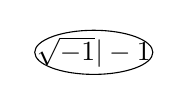
\begin{tikzpicture}
\draw (0,0) ellipse (0.75 and 0.28);
\node at (0,0) {$\unsure{\sqrt{-1}|-1}$};
\end{tikzpicture}
}
\margin{$-1$ (carré mod $p$)\qquad $p\equiv\uline{1}\quad(4)$}
\margin{$p$\qquad $p$}
\margin{$\left[\frac{-1}{p}\right]=-1$}
\margin{$\operatorname{TORS}($}

% Typescript, read in its own upright orientation.
\begin{center}
- 17 -
\end{center}

$|z_i|\leq r_i$ ; soit $M$ la borne supérieure des normes des termes de la série
pour $|z_i|=r_i$ $(1\leq i\leq p)$ ; on a donc
\[
\|\unsure{\mathbf c|C}_{n_1n_2\ldots n_p}\|\leq M/r_1^{n_1}\ldots r_p^{n_p}
\]
ce qui montre que la série entière
$(M(\frac{x_1}{r_1})^{n_1}\ldots(\frac{x_p}{r_p})^{n_p})$
est une majorante de la série donnée ; on observera que la somme de cette majorante
est $M/(1-\frac{x_1}{r_1})(1-\frac{x_2}{r_2})\ldots(1-\frac{x_p}{r_p})$
pour $|x_i|<r_i$ $(1\leq i\leq p)$.
Une autre majorante est la série obtenue par substitution de
$\sum_{i=1}^p\frac{x_i}{r_i}$ à $u$ dans la série géométrique $(Mu^n)$ ;
en effet, il est immédiat que le coefficient de $x_1^{n_1}\ldots x_p^{n_p}$
dans cette série est le produit d'un entier $\geq1$ et de
$M/r_1^{n_1}\ldots r_p^{n_p}$ ; cette nouvelle majorante a pour somme
$M/(1-\sum_{i=1}^p\frac{x_i}{r_i})$ dans un voisinage assez petit de l'origine.

\uline{2. Résolution des équations analytiques}.

THEOREME 1 .- \uline{Soient}
$f_i(x_1,\ldots,x_p\,;\,y_1,y_2,\ldots,y_p)$ $(1\leq i\leq q)$
$q$ \uline{fonctions holomorphes scalaires définies dans une partie ouverte}
$A$ \uline{de} $K^{p+q}$.

\uline{Soit} $(a_1,\ldots,a_p\,;\,b_1,\ldots,b_q)$ \uline{un point de}
$A$ \uline{tel que}
$f_i(a_1,\ldots,a_p\,;\,b_1,\ldots,b_q)=0$ \uline{pour} $1\leq i\leq q$,
\uline{et que le déterminant fonctionnel}
$\Delta=\det(\partial f_i/\partial y_j)$ \uline{soit}
$\neq0$ \uline{en ce point}.
\uline{Alors il existe un voisinage} $V$ \uline{de} $(a_1,\ldots,a_p)$
\uline{dans} $K^p$ \uline{et un système de} $q$ \uline{fonctions scalaires}
$u_i(x_1,\ldots,x_p)$ $(1\leq i\leq q)$
\uline{holomorphes dans} $V$, \uline{satisfaisant aux conditions}
$u_i(a_1,\ldots,a_p)=b_i$ $(1\leq i\leq q)$ \uline{et}
\[
(1)\qquad
f_i(x_1,\ldots,x_p\,;\,u_1(x_1,\ldots,x_p),\ldots,u_q(x_1,\ldots,x_p))=0
\quad(1\leq i\leq q)
\]
\uline{en tout point de} $V$.
\uline{En outre}, \uline{si} $v_i$ $(1\leq i\leq q)$ \uline{est un système de}
$q$ \uline{fonctions continues au point} $(a_1,\ldots,a_p)$,
\uline{définies dans un voisinage de ce point, et satisfaisant aux conditions}
$v_i(a_1,\ldots,a_p)=b_i$ $(1\leq i\leq q)$ \uline{et}

\scanpage{78}
% archive foliation: 77

\uline{Conclusion} Les catégories $\uline{\operatorname{Eq}}(C)$,
$C\in\operatorname{Ob}\underline B_0$, sont
\deleted{des \unsure{gr-catégories munies de structures}}
\inserted{munies canoniquement d'une structure de}
catégorie de Picard \uline{strictes}
\deleted{\unsure{commutatives}}.
\deleted{\unsure{Ils sont}}
Ces cat. de Picard sont \uline{canoniquement} équivalentes entre elles,
et peuvent donc s'identifier à une même catégorie de Picard
$\underline B$ (catégorie de Picard de \uline{Brandt}).
Donc $\underline B$ opère sur chaque $C$, et pour
$\unsure{C''|C},C'\in\operatorname{Ob}\underline B_0$,
la catégorie \deleted{\unsure{Hom}}
$\uline{\operatorname{Eq}}(C,C')$ est canoniquement munie d'une structure
de tors-catégorie sous $\underline B$. De façon précise,
\[
C'\longmapsto\uline{\operatorname{Eq}}(C,C')
\]
\[
\underline B_0\longrightarrow
\text{la catégorie des tors-catégories sous }\underline B
\]
est une équivalence de $2$-catégories.

Si on a un chgt de base
\diagram{
\begin{array}{ccc}
A&\longrightarrow&A'\\
\unsure{\cap}&&\unsure{\cap}\\
K&\unsure{\subset|-}&K'
\end{array}
}
et si les $C_{A'}$ satisfont les mêmes conditions que les $C$,
alors on a un hom de \deleted{\unsure{gr}} catégories de Picard
\[
\underline B\longrightarrow\underline B'
\]
et l'hom \deleted{\unsure{de base}}
\[
C\longrightarrow C_{A'}
\]
est compatible avec les opérations de $\underline B,\underline B'$ \ldots

\scanpage{79}
% archive foliation: 78; typescript printed page number follows
\begin{center}
- 16 -
\end{center}

ce qui prouve que la série considérée est absolument convergente pour
$\|u\|<1/5a$. Le fait que $(h(u))^2=e+u$ résulte de ce que la formule
$(1-\sum_{n=1}^{\infty}\binom{2n}{n}x^n)^2=1-4x$ est vraie lorsque
$E=K=\mathbb R$ (\uline{Fonct.var.réelle}, chap.III,§2)
(cf.n°2, remarque suivant la prop.2).

Reste à montrer que la fonction $g$ est la seule fonction continue et égale
à $e$ à l'origine, dont le carré soit $f$. Or, la relation $g^2-g_1^2=0$
s'écrit $(g-g_1)(g+g_1)=0$ puisque $E$ est commutative ; mais comme
$g(0)+g_1(0)=2e$, $g+g_1$ est inversible dans un voisinage de l'origine,
donc on a $g-g_1=0$ dans ce voisinage, ce qui achève la démonstration.

\begin{center}
§ 2. La méthode des majorantes.
\end{center}

\uline{1. Majorantes d'une série entière}.

DEFINITION 1.- \uline{Etant donnée une série entière}
$(\unsure{\mathbf c|C}_{n_1n_2\ldots n_p}z_1^{n_1}\ldots z_p^{n_p})$
\uline{à coefficients dans} $E$, \uline{par rapport aux variables}
$z_i\in K$ $(1\leq i\leq p)$,
\uline{on dit qu'une série entière}
$(C_{n_1n_2\ldots n_p}x_1^{n_1}\ldots x_p^{n_p})$
\uline{à coefficients \unsure{positifs}}
\uline{par rapport aux variables réelles} $x_i$ $(1\leq i\leq p)$,
\uline{est une majorante de \unsure{la} série entière donnée, si pour tout système d'exposants}
$(n_1,n_2,\ldots,n_p)$, \uline{on a}
$\|\unsure{\mathbf c|C}_{n_1n_2\ldots n_p}\|\leq C_{n_1n_2\ldots n_p}$.

Il est clair que la somme (resp. le produit) de majorantes de deux séries
entières est une majorante de la somme (resp. du produit) de ces deux séries.

Si une majorante d'une série entière est sommable pour
$x_1=r_1>0,\ldots,x_p=r_p>0$, il est clair que la série entière donnée
est absolument sommable dans le polycylindre fermé défini par
$|z_i|\leq r_i$ $(1\leq i\leq q)$.
Inversement, supposons qu'une série entière
$(\unsure{\mathbf c|C}_{n_1\ldots n_p}z_1^{n_1}\ldots z_p^{n_p})$
soit absolument sommable dans le polycylindre fermé

\scanpage{84}
% archive foliation: 83
\margin{$\unsure{c}$}

$\mathcal M$ catégorie motivique \inserted{\unsure{$k$ un corps}},
de gerbe $\mathcal G$. Supposons que le lien $\mathcal L$ de $\mathcal G$
soit \uline{commutatif}, donc correspond à un groupe algébrique
\inserted{comm de type multiplicatif} $G$ sur $\mathbb Q$.
Ainsi, $G^\circ$ est un tore. Soit $E$ un motif ``fidèle''.
\deleted{et \unsure{par $E$ un foncteur}}
\inserted{Alors} $G$ opère sur $E$, considéré comme
\deleted{\unsure{objet}}\inserted{section}
de la catégorie fibrée $\operatorname{HOM}(\mathcal G,\uuline{\unsure{\mathrm{Proj}}})$,
et en particulier $G(\mathbb Q)$ opère sur $E$ donc
\[
G(\mathbb Q)\overset{\varphi}{\hookrightarrow}\operatorname{End}_{\mathcal M}(E).
\]
D'ailleurs,
\deleted{les éléments de $G(\mathbb Q)$}
\deleted{Soit $U=\operatorname{Ker}(G^\circ\longrightarrow G_m)$,
alors $U$ opère}
\deleted{\unsure{sur}}
Choisissons une forme de polarisation sur $E$, d'où une structure
d'Algèbre de Riemann sur $A=\operatorname{End}_{\mathcal M}(E)$,
et \unsure{on trouve} que pour $u\in G(\mathbb Q)$,
\[
\varphi(u)\varphi(u)^{\deleted{\unsure{*}}\inserted{'}}=
\varepsilon(u)\unsure{1|1_E}\deleted{\unsure{*}}.
\]
[En particulier, si $u\in\operatorname{Ker}\varepsilon$,
\inserted{$U=$}
on aura $\varphi(u)\varphi(u)'=\operatorname{id}$.]
Donc l'algèbre engendrée par les $\varphi(u)$ dans $A$ est auto-adjointe,
et $U(\mathbb Q)$ apparaît comme un s-groupe du
``groupe unitaire'' de $A$, formé des unités $u$ telles que $uu'=1$.
\deleted{Plus précisément}
Or ce \inserted{dernier} groupe est
\inserted{\unsure{fermé dans $\operatorname{Units}(A/\mathbb Q)$} et}
\unsure{un} \uline{donc} \uline{compact}.
On \unsure{trouve} que $U^\circ$ est un \uline{tore compact}.

\scanpage{85}
% archive foliation: 84; reused printed/typescript excerpt, oppositely oriented

où $p_{X'}$ désigne le morphisme structural $X'\quad X$.
D'autre part, pour donner un sens à 4.1. (ii) et justifier sa démonstration
indiquée de 4.1., il y a lieu d'introduire un univers \quad tel que \quad
\unsure{,}
et considérer les faisceaux intervenant dans les formules \unsure{4.1.}
\unsure{(ii)}
comme des faisceaux à valeurs dans \quad -(Ens).
% Blank spaces in the copy at the structural morphism and universe notation;
% no arrow or universe letter has been supplied from mathematical expectation.

\uline{Proposition \unsure{4I1.|4.1.}} (i) Le foncteur
$u^{\unsure{X|*}}$ est pleinement fidèle, donc pour tout faisceau $G$
sur $X_{\text{ét}}$, l'homomorphisme canonique
\[
G\qquad u_{\unsure{X|*}}u^{\unsure{X|*}}(G)
\]
est un isomorphisme.

(ii) Soient $G$ (resp. $F$) un faisceau abélien sur $X_{\text{ét}}$
(resp. $(\mathrm{Sch})/X$).
Alors les homomorphismes canoniques (définis par exemple comme
edge-homomorphismes de la suite \unsure{spectrahe|spectrale} de Leray V 5.5.1.)
suivants \unsure{sontx|sont} des isomorphismes:
\[
H^{\unsure{*}}(X_{\text{ét}},F\,u)\simeq
H^{\unsure{*}}((\mathrm{Sch})/X,F)
\]
\[
H^*(X_{\text{ét}},G)\simeq
H^{\unsure{*}}((\mathrm{Sch})/X,u^{\unsure{*}}(G)).
\]
En effet, le foncteur $u$ est un comorphisme (VI 7.3.6.) et on peut alors
appliquer VI 7.3.7. et VI 7.3.9.

\scanpage{86}
% archive foliation: 85

On peut préciser, en introduisant l'algèbre engendrée par
\deleted{\unsure{$A$}} $G(\mathbb Q)$ dans $A$, soit $B$.
On sait que $B=\prod L_i$, chaque $L_i$ ext. quadratique d'un corps
de nb $K_i$ tt. réel.
($K_i$ déterminé \unsure{uniquement}
\deleted{\unsure{par la condition}}\inserted{dans $L_i$}
comme \unsure{l'un des s/c tt. réels} de $L_i$),
l'involution est donnée sur $L_i$ par la conjugaison p.r. à $K_i$
(i.e. la conjugaison complexe ordinaire, si $L_i\subset\mathbb C$),
la trace est proportionnelle, sur chaque $L_i$, à la trace ordinaire.
Ainsi $B^*$ n'est autre que $H(\mathbb Q)$, où
\[
H=\prod_i\left(\prod_{L_i/\mathbb Q}G_{m\,L_i}\right)
\]
et le \unsure{groupe|gr.} unitaire $B^{*u}$ n'est autre que \unsure{le} \deleted{\unsure{groupe}} des pts rationnels de
\[
H^u=\prod_i\left(\prod_{K_i/\mathbb Q}\unsure{\Gamma_i|\mathcal T_i}\right)
\]
où $\unsure{\Gamma_i|\mathcal T_i}$ est la forme tordue de $G_m$ sur $K_i$
définie par l'extension quadratique $L_i$ de $K_i$.
\deleted{[}\deleted{Ainsi}
Cela met en évidence que $H^u$ est un tore ``compact'',
\deleted{\unsure{donc il est}}
(de nature d'ailleurs assez particulière!), et aussi $U^\circ$ comme
sous-tore de ce dernier \ldots

NB. Il convient de déterminer $\varepsilon:G\longrightarrow G_m$
en termes des \unsure{hom. normes} sur les $L_i$, et
$j:G_m\longrightarrow G$ \inserted{de même \ldots}
